\documentclass[11pt, oneside]{article}   	% use "amsart" instead of "article" for AMSLaTeX format
\usepackage{geometry}                		% See geometry.pdf to learn the layout options. There are lots.
\geometry{letterpaper}                   		% ... or a4paper or a5paper or ... 
%\geometry{landscape}                		% Activate for rotated page geometry
%\usepackage[parfill]{parskip}    		% Activate to begin paragraphs with an empty line rather than an indent
\usepackage{graphicx}				% Use pdf, png, jpg, or eps§ with pdflatex; use eps in DVI mode
								% TeX will automatically convert eps --> pdf in pdflatex		
\usepackage{amssymb}

%SetFonts

%SetFonts

\setlength\parindent{0pt}

\title{Why Use Logarithmic Returns?}
\author{Lucas Louca}
%\date{}							% Activate to display a given date or no date
\usepackage{amsmath}

\begin{document}
\maketitle
%\section{}
%\subsection{}

\section{Preliminaries}
Calculating simple returns is done using:
\begin{equation}
R=\frac{P_i - P_j}{P_j}
\end{equation}

To find the total return over a period $T$ with $n$ sub-periods, we need to compound the growth for each sub-period, as shown here:
\begin{equation}
	P_f = P_0(1+R_1)(1+R_2)...(1+R_n)
\end{equation}	
with: 
\begin{center}
	\begin{itemize}
		\item $P_f$ - final Price
		\item $P_0$ - initial Price
		\item $R_x$ - Return for each sub-period.
	\end{itemize}
\end{center}	

If each return $R_x$ were identical, we could write this in a simplified exponential form:
\begin{equation}
	P_f =P_0(1+R_n)^n
\end{equation}	
But, the return in each sub-period is rarely identical, so compounding in this manner is impossible. For this reason, we turn our attention to logarithmic returns. Logarithmic returns measure the rate of exponential growth. Instead of measuring the percent of price change for each sub-period, we measure the exponent of its natural growth during that time. Later, we can add each sub-period's exponential growth to get the total growth for the period $T$.
\\
\\
If you invest an amount  $P_1$ for one year at an $r\%$ interest rate, at the end of the year you'll have an amount:
\begin{equation}
	P_2 = P_1(1+r)
\end{equation}
For example, with a $4\%$ return, $P_2 = 1.04P_1$. Sometimes your interest might be compounded, for example, you get your money back plus $2\%$ at the end of six months, and then can earn $2\%$  interest on both your original principal as well as on the  first six month's interest: 
\begin{equation}
	P_2 = P_1(1+\frac{r}{2})(1+\frac{r}{2}) = P_1(1+\frac{r}{2})^2
\end{equation}
Similarly, compounded quarterly you will get:
\begin{equation}
	P_2 = P_1(1+\frac{r}{4})^4
\end{equation}
It turns out the formula converges to a particular function as the frequency of compounding $n$ gets arbitrarily large, this limit being:
\begin{equation}
	\displaystyle{\lim_{x \to \infty}}(1 + \frac{r}{n})^n = e^r
\end{equation}
Thus if you earn $r\%$ interest that is \emph{compounded continuously}, at the end of the year your money will be:
\begin{equation}
	P_2 = P_1\displaystyle{\lim_{x \to \infty}}(1 + \frac{r}{n})^n = P_1e^r
\end{equation}
or grown by a factor:
\begin{equation}
	\frac{P_2}{P_1} = e^r
\end{equation}
where $e$ is a special number (approximately equal to $2.72$). Taking the natural logarithm is just the inverse of the above operation: 
\begin{equation}
	r = ln(\frac{P_2}{P_1})
\end{equation}
$r = ln(\frac{P_i}{P_j})$ is referred to as the \emph{logarithmic return}. Often times you will see the following equation:
\begin{equation}
	ln(R_i + 1) = ln(\frac{P_i}{P_j})
\end{equation}
This is easy to derive:
\begin{align}
	\begin{split}
		R_i & = \frac{P_i - P_j}{P_j} \\
		R_i & = \frac{P_i}{P_j} - 1\\
		R_i + 1 &  = \frac{P_i}{P_j}\\
		\rightarrow\\
		ln(R_i + 1) & = ln(\frac{P_i}{P_j}) \\ 
		&  = ln(P_i) - ln(P_j)\\
	\end{split}
\end{align}

\section{Property 1:  Symmetry}
Simple returns are not \emph{symmetric}: positive and negative percent ordinary returns of equal magnitude do not cancel each other out and result in a net change. For example, if your portfolio goes up by $50\%$ (say from $\$100$ to $\$150$) and then declines by $50\%$ (say from $\$150$ to $\$75$), you're not back where you started. If you calculate your average percentage return (in this case, $0\%$), that's not a particularly useful summary of the fact that you actually ended up $25\%$ below where you started. That is, if you just calculate the average like so:
\begin{equation}
	\frac{(\frac{150-100}{100} + \frac{75-150}{150})}{2} = 0\%
\end{equation}
the arithmetic average suggests that you have earned an average of $0\%$. But in reality you lost $25\%$. Do you see the problem here? Arithmetic return has a positive bias. 
\\
\\
Logarithmic returns are useful for mathematical finance. One of the advantages is that the logarithmic returns are symmetric. While ordinary returns are not, logarithmic returns of equal magnitude but opposite signs will cancel each other out. This means that an investment of $\$100$ that yields a simple return of $50\%$ followed by a simple return of $-50\%$ will result in $\$75$, while an investment of $\$100$ that yields a logarithmic return of $50\%$ followed by a logarithmic return of $-50\%$ will come back to $\$100$. 
\\
\\
Consider this example. You have invested $\$100$ in a stock in year 1, it grows to  $\$200$ in year 2 giving you a return of $100\%$. In year 3 the stock price comes back to $\$100$ from  $\$200$ giving you a negative return of $50\%$. What do you think is the average return? If you calculate the average like so:
\begin{equation}
	\frac{(100\% - 50\%)}{2} = 25\%
\end{equation}
the arithmetic average is suggesting that you have earned an average of $25\%$. But in reality you have earned $0\%$. That's not a particularly useful summary. On the other hand, the average log return is indeed $0\%$ which is more informative:
\begin{center}
  \begin{tabular}{ | c | c | c | c | }
    \hline
    Period & Price & Simple Return & Log Return \\ \hline
    Year 1 & $100$ & - & - \\ \hline
    Year 2 & $200$ & $100\%$ & $69\%$ \\ \hline
    Year 3 & $100$ & $-50\%$ & $-69\%$ \\
    \hline
  \end{tabular}
\end{center}
See the symmetry of the log returns in the above table?

\section{Property 2:  Time-additivity}
Simple returns are not \emph{additive} over time. Adding returns for multiple periods does not yield the total return over the total length of time. In other words, simple returns don't satisfy the property of \emph{time consistency}. For example, if your portfolio goes from $\$10$ to $\$11$ in one year and then to $\$12$ the next year, your annual simple returns would be $10.0\%$ and $9.09\%$ respectively. Adding those returns up would sum up to $19.09\%$, which is not your actual return of $20\%$.
\\
\\
On the other hand, logarithmic returns are \emph{additive} over time. Consider an ordered sequence of $n$ trades. Calculating the compounding return, which is the running return of this sequence of trades over time:
\begin{equation}
	(1+R_1)(1+R_2)...(1+R_n) = \displaystyle{\prod_{i}^{n}} (1 + R_i)
\end{equation}
where $R_i$ is the return for each period. Taking the natural logarithm of this would give us:
\begin{align*}
	\begin{split}
	ln(\displaystyle{\prod_{i}^{n}} (1 + R_i)) 
	& = \displaystyle{\sum_{i}^{n}} ln(1 + R_i) \\ 
	& = ln(1 + R_1) + ln(1 + R_2) + \dots + ln(1 + R_n) \\
	& = ln(\frac{P_1}{P_0}) + ln(\frac{P_2}{P_1}) + ln(\frac{P_3}{P_2}) + \dots + ln(\frac{P_{n-1}}{P_{n-2}}) + ln(\frac{P_n}{P_{n-1}}) \\
	& = ln(P_1) - ln(P_0) + ln(P_2) - ln(P_1) + \dots + ln(P_n) - ln(P_{n-1}) \\
	& = ln(P_n) - ln(P_0)
	\end{split}
\end{align*}
As we can see, if we sum up the logarithmic returns $ln(\frac{P_i}{P_j})$ for each period, we end up with $ln(P_n) - ln(P_0) = ln(\frac{P_n}{P_0})$. In other words, the compound return over $n$ periods is merely the difference in log between initial and final periods. 
\\
\\
Back to our portfolio example, if your portfolio goes from $\$10$ to $\$11$ in one year and then to $\$12$ the next year, your logarithmic return $r$ over the period of two years would be:
\begin{equation}
	r = ln(P_2) - ln(P_0) = ln(12) - ln(10) = 0.18
\end{equation}
which is the same as summing the logarithmic returns of each individual period:
\begin{equation}
ln(\frac{P_1}{P_0}) + ln(\frac{P_2}{P_1})  = ln(\frac{11}{10}) + ln(\frac{12}{11}) = 0.18
\end{equation}
In terms of algorithmic complexity, this simplification reduces $\mathcal{O}(n)$ multiplications to $\mathcal{O}(1)$ additions. This is a huge win for moderate to large $n$. 
\\
\\
$P_2$ can also be expressed as $e$ raised to the logarithmic return $r$:
\begin{align*}
	\begin{split}
		P_2 & = P_0 (1+R_1)(1+R_2) \\
		& = P_0  \displaystyle{\prod_{0}^{2}} (1 + R_i) \\ 
		& = P_0 e^{ln( \displaystyle{\prod_{0}^{2}} (1+R_i))} \\
		& = P_0 e^{ln(\frac{P_2}{P_0})} \\
		& = P_0 e^{ln(\frac{12}{10})} \\
		& = 12
	\end{split}
\end{align*}

And, because the logarithmic returns are additive, the arithmetic mean of log returns is much more informative: the average log return, times the number of sub-periods, tells us the exact total compounded return over the period of study.

\section{Property 3:  Viewing Economic Data}
To refresh your memory of school math, logs are just another way of writing exponential equations, one that allows you to separate the exponent on one side of the equation. The equation $2^4 = 16$ can be rewritten as $log_2 16 = 4$ and pronounced "log to the base 2 of 16 is 4." The equation $y = log_b (x)$ means that $y$ is the power or exponent that $b$ is raised to in order to get $x$.
\\
\\
On a linear scale, a change between two values is perceived on the basis of the \emph{difference} between the values. Thus, for example, a change from $1$ to $2$ would be perceived as the same amount of increase as from $4$ to $5$. On a logarithmic scale, a change between two values is perceived on the basis of the \emph{ratio} of the two values. That is, a change from $1$ to $2$ (ratio of $1:2$) would be perceived as the same amount of increase as a change from $4000$ to $8000$ (also a ratio of $1:2$). You can see that log scales allow a large range to be displayed without small values being compressed down into bottom of the graph. Log scales respond to skewness towards large values.
\\
\\
Consider this example. The revenue for Boeing in 2010 was about $2^6$ billion dollars while the revenue for Ford Motor was about $2^7$. In a linear scale, the revenue for Ford is the revenue for Boeing plus the difference between these two revenues. We call this additive. Since $2^6 = 64$ and $2^7 = 128$, we see that the difference is about $64$ billion dollars. In a log scale, the difference is multiplicative. Since $2^7 = 2^6 \cdot 2$, we see that the revenues for Ford Motor are about double those for Boeing. This is what we mean by saying that we use logarithmic scales to show multiplicative factors.
\\
\\
Logarithms are often a much more useful way to look at economic data. For example, here is a graph of the SP500 index going back to 1871. Plotted on arithmetic scale, one can see nothing in the  first century, whereas the most recent decade appears insanely volatile.
\begin{center}
	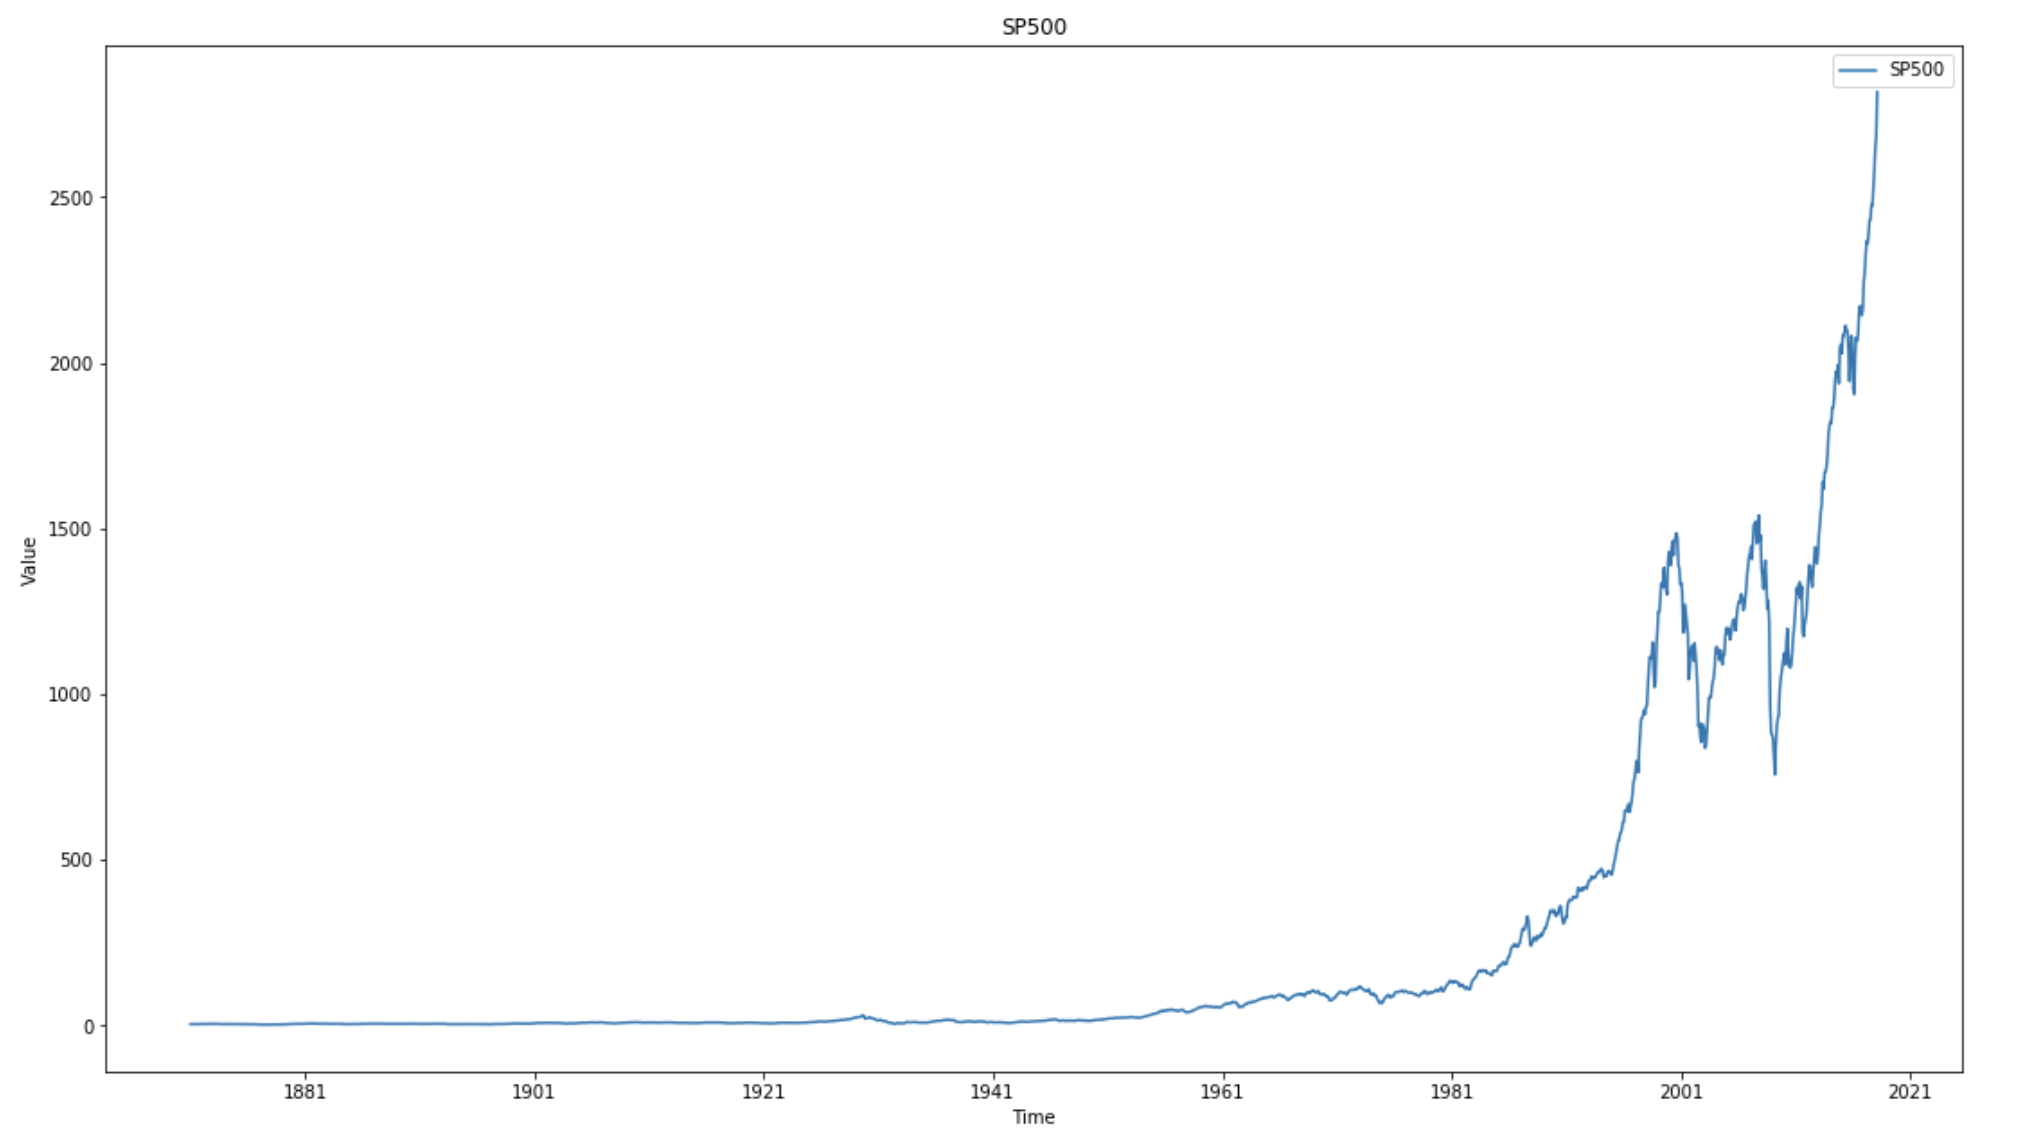
\includegraphics[scale=0.4]{sp500_arithmetic.png}
\end{center}
On the other hand, if you plot these same data on a log scale, you do no longer consider absolute change, but relative change. That is, $log_2(16) - log_2(8) = log_2(2000) - log_2(1000)$. Plotted this way, it's clear that, in percentage terms, the recent volatility of stock prices is actually modest relative to what happened in the Great Depression in the 1930's.
\begin{center}
	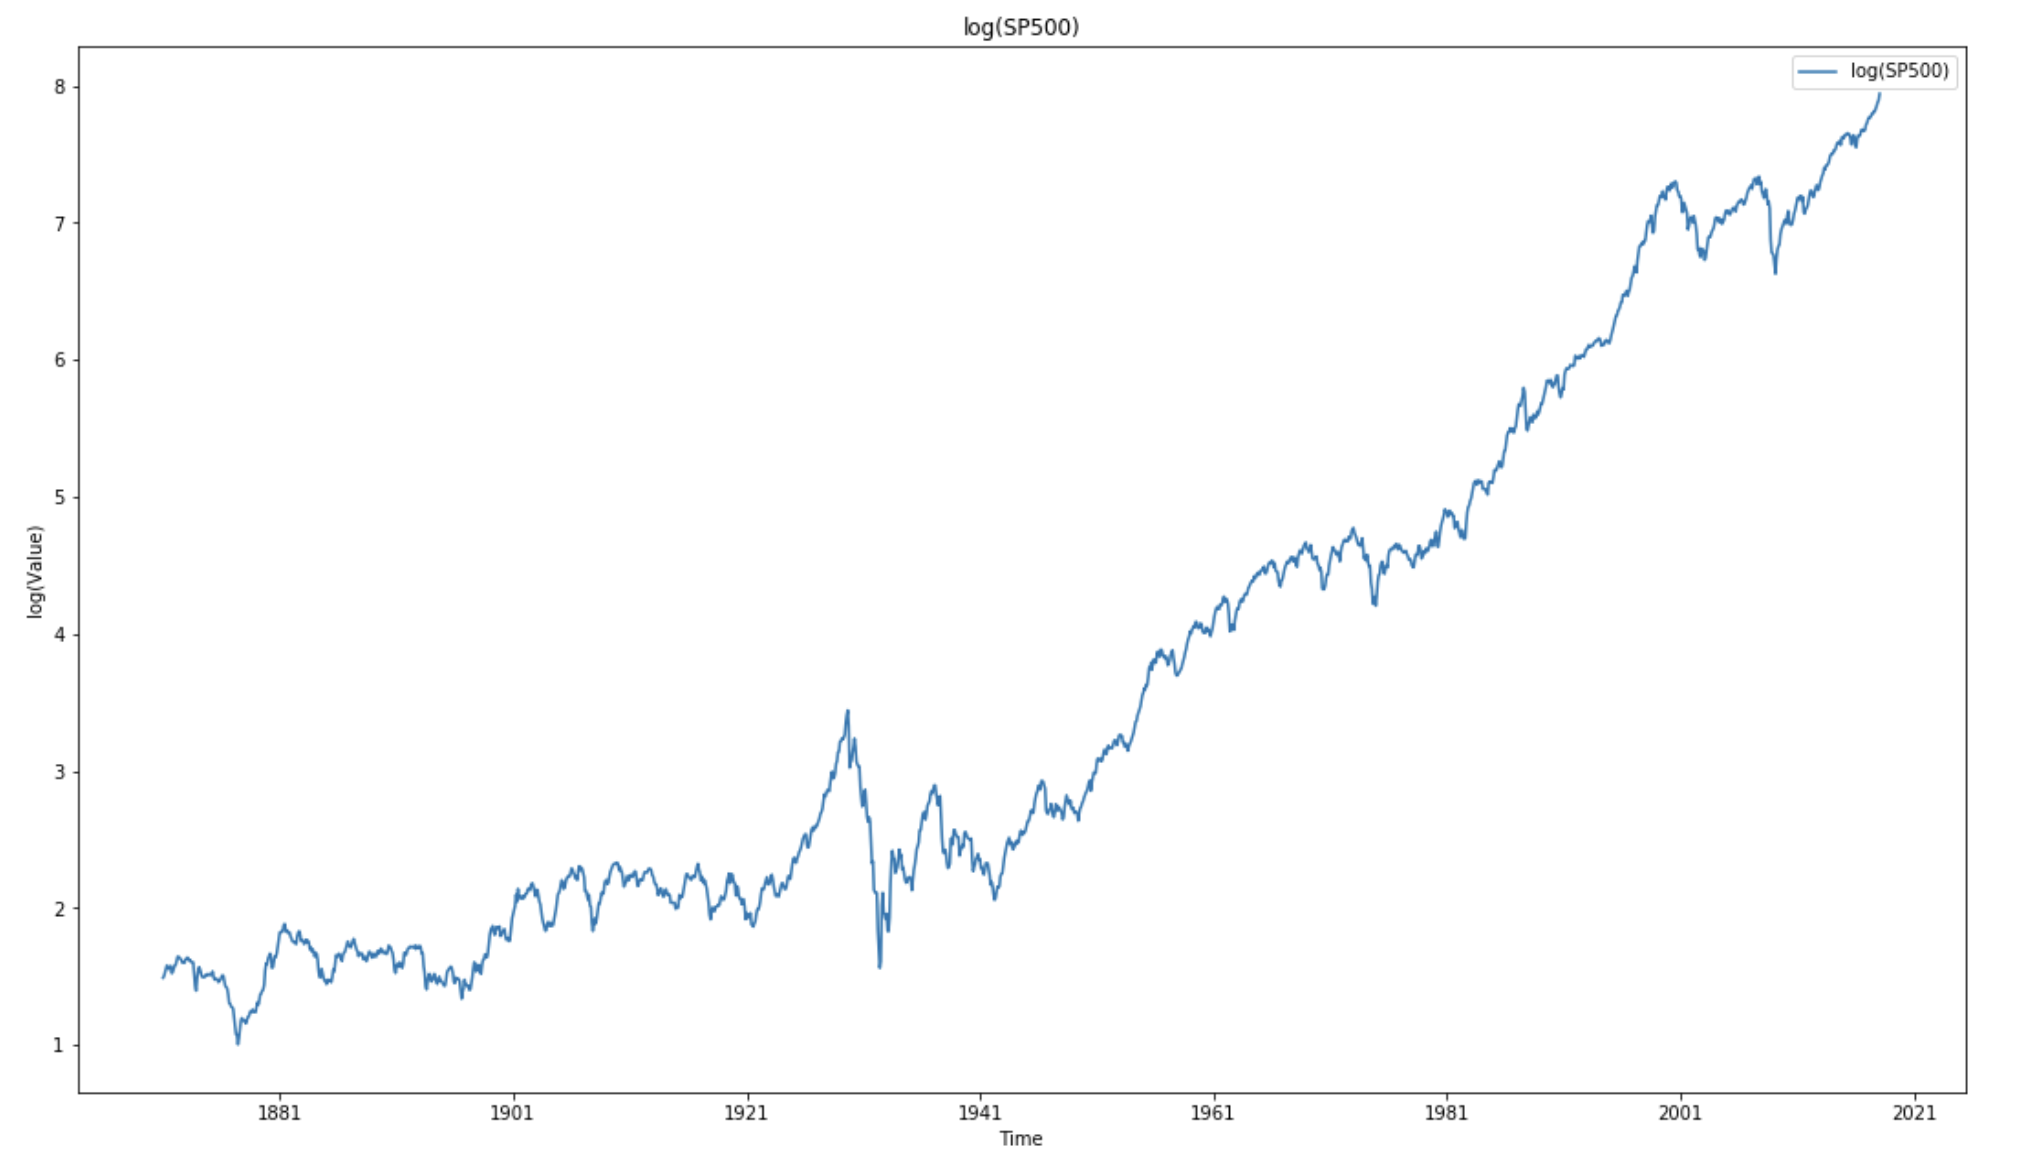
\includegraphics[scale=0.4]{sp500_log.png}
\end{center}

\end{document}  